\documentclass[a4paper,12pt]{article}
\usepackage{polski}
\usepackage[utf8]{inputenc}
\usepackage[left = 3cm, right = 3cm, top = 2cm, bottom = 2cm]{geometry}
\usepackage{enumerate}
\usepackage{amssymb}		% pakiet do symboli
\usepackage{mathtools}		% pakiet do matmy (rozszerza amsmath)
\usepackage{enumitem}		% punktowanie (a), (b), ...
\usepackage{nopageno}		% brak numerow stron
\usepackage{graphicx}		% wstawianie obrazkow
\usepackage{float}			% wstawianie obrazkow w dowolnym miejscu
\usepackage{caption}
\usepackage{esdiff}         % pochodne \diff{}{}
\usepackage{listings}
\usepackage{xcolor}
\usepackage{adjustbox}
%\usepackage[none]{hyphenat} % usunięcie łamania wyrazów na końcu linii

% nowe komendy dla wygodniejszego pisania :)

\newcommand{\floor}[1]{\left\lfloor #1 \right\rfloor}	% podłoga
\newcommand{\ceil}[1]{\left\lceil #1 \right\rceil}		% sufit
\newcommand{\fractional}[1]{\left\{ #1 \right\}}		% część ułamkowa {x}
\newcommand{\abs}[1]{\left| #1 \right|}					% wartosc bezwzgledna / moc
\newcommand{\set}[1]{\left \{ #1 \right \}}				% zbiór elementów {a,b,c}
\newcommand{\pair}[1]{\left( #1 \right)}				% para elementów (a,b)
\newcommand{\Mod}[1]{\ \mathrm{mod\ #1}}				% lekko zmodyfikowane modulo
\newcommand{\comp}[1]{\overline{ #1 }} 					% dopełnienie zbioru 
\newcommand{\annihilator}{\mathbf{E}}					% operator E
\newcommand{\seqAnnihilator}[1]{\annihilator \left\langle #1 \right\rangle} % E(a_n)
\newcommand{\sequence}[1]{\left\langle #1 \right\rangle} % <a_n>
\DeclareMathOperator{\lcm}{lcm}							% obsługa lcm w mathmode

% styl do kodu
\lstdefinestyle{code}{%
basicstyle=\ttfamily\small,
commentstyle=\color{green!60!black},
keywordstyle=\color{magenta},
stringstyle=\color{blue!50!red},
showstringspaces=false,
numbers=left,
numberstyle=\footnotesize\color{gray},
numbersep=10pt,
tabsize=4,
rulecolor=\color{red},
breaklines=true
}

\newcommand{\code}[1]{\lstinline[style=code]{#1}} % kod inline

\begin{document}
\noindent \textbf{Matematyka dyskretna L, Lista 11 - Tomasz Woszczyński}\newline

\noindent \newline \textbf{Zadanie 2} \newline
Topologiczne porządkowanie wierzchołków acyklicznego digrafu. Niech $D$ będzie digrafem
acyklicznym, tzn. $D$ nie zawiera cykli skierowanych. Podaj algorytm, który w czasie
$O(n + m)$ porządkuje wierzchołki digrafu w taki sposób, że po uporządkowaniu, jeśli
$(i, j)$ jest krawędzią skierowaną w $D$, to $i < j$. \\

\noindent Poniższy algorytm stopniowo usuwa wierzchołki o stopniu wchodzącym $0$ (a więc nie 
wchodzi w nie żadna krawędź). Kolejność usuwania wierzchołków jest szukanym rozwiązaniem, 
nazwy  takich wierzchołków będą wypisywane. Gdy po usunięciu wszystkich wierzchołków o 
$\deg_{\text{in}}(v) = 0$ zostaną jakieś wierzchołki, oznacza to, że w grafie istnieje cykl, 
a więc podany graf $D$ nie był acykliczny.

\begin{lstlisting}[style=code, language=python]
def topological_sort(D):
    Q = {queue of vertices with deg_in == 0}

    while Q is not empty:
        remove v from the front of Q
        print v

        for each edge e to u (neighbour of v):
            remove e from D
            if u has no more incoming edges:
                push u to Q

    if G has vertices:
        print "there are cycles in D (which is not acyclic)"
\end{lstlisting}

\noindent Taki algorytm nie wyznacza jednoznacznie takiego porządku. Spowodowane jest to
tym, w jaki sposób tworzymy kolejkę na samym początku algorytmu. Za przykład niech posłuży
nam poniższy graf. Kolejkę wierzchołków o stopniu wchodzącym $0$ możemy stworzyć na kilka
sposobów, na przykład $Q_1 = \{ 2, 1, 0\}$ czy $Q_2 = \{ 1, 0, 2 \}$ (oczywiście to nie są
wszystkie możliwości). Ponadto, usuwając kolejne krawędzie (np. od wierzchołka $2$), możemy
je wybierać w różnej kolejności. 

\begin{figure}[H]
    \centering
    $\vcenter{\hbox{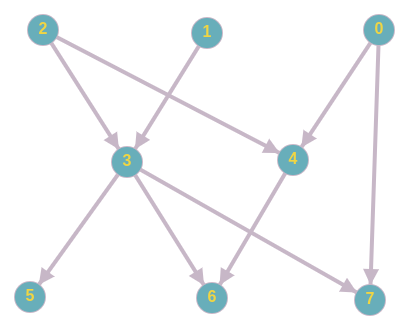
\includegraphics[width=.5\textwidth]{Rysunki/l11z2.png}}}$
\end{figure}

\noindent Wtedy dla $Q_1$ możemy otrzymać np. $\{ 2, 1, 0, 3, 4, 5, 7, 6 \}$, a dla $Q_2$
możemy uzyskać $\{ 1, 0, 2, 4, 3, 5, 6, 7 \}$. Tak jak wspomniałem wyżej, nie są to jedyne
możliwości.

\newpage
\noindent \textbf{Zadanie 3} \newline
Digraf, w którym każda para różnych wierzchołków jest połączona dokładnie jedną krawędzią
skierowaną, nazywamy turniejem (jest to skierowany graf pełny). Pokaż, że w każdym turnieju
istnieje wierzchołek, z którego można dojść do każdego innego wierzchołka po drodze 
o długości co najwyżej $2$. \\

\noindent Weźmy wierzchołek $v$ o największej ilości łuków wychodzących, a w przypadku gdy
istnieje kilka takich łuków, wybierzmy dowolny z nich. Załóżmy, że liczba łuków wychodzących
jest mniejsza od liczby krawędzi tego grafu, w przeciwnym wypadku sytuacja byłaby trywialna,
gdyż do każdego wierzchołka możnaby było dojść po drodze długości 1, co kończyłoby dowód. \\

\noindent Załóżmy nie wprost, że istnieje wierzchołek $u$, do którego nie można dojść z $v$
w po ścieżce długości $2$. Wierzchołek $u$ ma krawędzie skierowane do każdego innego
wierzchołka: są to wierzchołki, do których można dojść z $v$ jednym ruchem oraz $v$. Aby
nie można było dojść do tego wierzchołka $u$ w dwóch ruchach, to wymienione przed chwilą
krawędzie musiałyby wychodzić z $u$ - to oznaczałoby, że $u$ ma więcej łuków wychodzących 
niż $v$, ponieważ wychodziłyby z niego krawędzie skierowane do wierzchołków wychodzących z $v$
oraz do $v$. Dochodzimy więc do sprzeczności, gdyż 
\[
    \deg_{\text{out}}(v) + 1 = \deg_{\text{out}}(u) 
\]
lecz wcześniej założyliśmy, że wybrany wierzchołek $v$ ma najwięcej łuków wychodzących.
Przeczy to założeniu, że nie ma wierzchołka z większą ilości krawędzi wychodzących z $v$,
czyli nie ma wierzchołka do $u$, do którego nie da się dojść w dwóch krokach.

\noindent \newline \textbf{Zadanie 4} \newline
\textbf{Pierwsza część:} Podaj warunek konieczny na to, by graf dwudzielny był grafem 
hamiltonowskim. \\

\noindent Dla grafu dwudzielnego $G$, aby był on grafem hamiltonowskim, a więc grafem,
który zawiera cykl przechodzący przez każdy wierzchołek dokładnie jeden raz,
dwa rozłączne zbiory $A$ i $B$, takie że $A \cup B = V(G)$ i $A \cap B = \emptyset$,
muszą spełniać własność $\abs{A} = \abs{B}$. Aby to udowodnić, załóżmy bez straty ogólności, 
że $\abs{A} > \abs{B}$. Załóżmy, że graf $G$ zawiera cykl Hamiltona, który zaczyna się 
w wierzchołku $u \in B$. Po przejściu $2 \abs{B}$ krawędzi, pozostanie $\abs{A} - \abs{B}$ 
nieodwiedzonych wierzchołków w $A$, co oznacza, że w grafie $G$ nie może powstać cykl 
hamiltonowski. \\

\noindent \textbf{Druga część:} Zaczynając od dowolnego pola, czy można obejść ruchem skoczka 
szachowego wszystkie pola szachownicy $5 \times 5$, każde dokładnie raz, i wrócić do punktu 
początkowego? Odpowiedź uzasadnij. \\

\noindent Szukając zamkniętej ścieżki konika szachowego należy przyjrzeć się temu, w jaki
sposób odbywa się ruch skoczka po szachownicy. Zawsze przechodzi on z pola jednego koloru
na pole innego koloru. Oznacza to, że zaczynając na polu białym, konik musiałby wylądować
w ostatnim ruchu na tym samym polu, analogicznie w przypadku pola czarnego. Oznacza to, 
że ścieżka zamknięta skoczka istnieje tylko dla szachownic o parzystej liczbie pól, a więc
dla szachownicy $5 \times 5$ nie istnieje żadna taka ścieżka zamknięta.

\newpage
\noindent \textbf{Zadanie 5} \newline
Dana jest kostka sera $3 \times 3 \times 3$. Mysz rozpoczyna jedzenie kostki od dowolnego
rogu. Po zjedzeniu jednego pola przenosi się do kolejnego mającego wspólną ścianę z ostatnio
zjedzonym. Czy możliwa jest sytuacja, aby mysz jako ostatnie zjadła środkowe pole? \\

\noindent Taka sytuacja nie jest możliwa. Pokolorujmy wszystkie kostki na biało-czarno 
i załóżmy, że rogi są koloru czarnego. Mamy wtedy 14 kostek czarnych i 13 kostek białych. 
Z założenia z zadania, możemy przechodzić tylko do sąsiednich kostek, co w naszym przypadku oznacza przejścia z kostek białych do czarnych lub na odwrót. Kostka w samym środku jest
biała, a więc jeśli zaczniemy przechodzić od niej (możemy zacząć wędrówkę od wewnętrznej
kostki, gdyż tę ścieżkę możemy wtedy "odwrócić"), trasa będzie wyglądać następująco:
\[
    \underbrace{B \to C \to B \to C \to \dots \to B \to C}_{\text{13 ruchów między
    różnymi kolorami}} \to {}?
\]
Niestety, ostatnią kostką jaka nam została, jest kostka $C$, jednak ruch między kostkami
tego samego koloru jest niedozwolony. Oznacza to, że mysz nie będzie mogła zjeść środkowego
pola jako ostatniego.

\end{document}